\chapter{Background}
\label{chap:background}

\section{The QUIC Protocol}
\label{sec:the-quic-protocol}

\section{eBPF}
\label{sec:bpf}
\ac{eBPF}, also simply known as \ac{BPF}, is a Linux-native in-kernel bytecode language and virtual machine that allows for programmable, event-driven execution across many of the kernel's subsystems. It represents an evolution from \ac{cBPF}, which also offers an in-kernel bytecode language and virtual machine but with fewer capabilities. The work flow for creating an \ac{eBPF} program typically entails writing the program in a subset of C, compiling it using a tool like LLVM, writing the user space loader program, and finally loading and attaching the program. Once a specific event occurs, the \ac{eBPF} program will subsequently be invoked. Finally, because it is a Linux-native technology, \ac{BPF} comes packaged with every kernel version since 3.18~\cite{starovoitov2014bpf}.

\subsection{Instruction Set}
\label{subsec:instruction-set}
\ac{BPF} is a general purpose \ac{RISC} architecture which can be used as a compilation target for
compiler back ends like LLVM. Typically written in a subset of C that does not allow features such as arbitrary loops, unbounded recursion, and arbitrary memory accesses, \ac{BPF} bytecode is loaded by the kernel at runtime and is later \ac{JIT} compiled into native opcodes for better performance. This approach allows the kernel to become programmable without having to cross the user-kernel space boundary. This is incredibly advantageous because it offers a flexible new way of gaining visibility into the Linux kernel as well as boosting data path performance by enabling data handling at the earliest possible stages. Moreover, BPF programs can be atomically updated at runtime without requiring a kernel restart, allowing for dynamic changes throughout a program's lifecycle.

\ac{BPF} consists of eleven 64 bit registers with 32 bit subregisters. It also contains a 512 byte stack space and a program counter. Each of the eleven registers are named \texttt{r0 - r10}, and the default operating mode is 64 bits. The 32 bit subregisters are only accessible through ALU operations. Table~\ref{tab:ebpf_registers} shows the BPF calling convention.

\begin{table}[h]
    \centering
    \begin{tabular}{c c p{6cm}}
        \toprule
        Register & Type     & Description \\
        \midrule
        r0       & R/W      & Exit value for BPF program. \\
        r1-r5    & R/W      & Scratch registers; hold arguments to the kernel helper function. \\
        r6-r9    & R/W      & Callee-saved scratch registers. \\
        r10      & Read-Only & Frame pointer for accessing the BPF stack. \\
        \bottomrule
    \end{tabular}
    \caption{eBPF Register Overview}
    \label{tab:ebpf_registers}
\end{table}

Because of the simple nature of \ac{BPF}'s calling convention, it can map directly to \texttt{x86\_64} and \texttt{arm64}, which greatly benefits the \ac{JIT} compiler given that it needs only to issue a single call instruction when placing function arguments.

\subsection{Helper Functions}
\label{subsec:helper-functions}
Depending on the hook point, a given \ac{eBPF} program will have access to a number helper functions, which provide assistance in retrieving and pushing data to the kernel. Using the registers defined in Table~\ref{tab:ebpf_registers}, a typical helper function signature will take a form similar to \texttt{u64 fn(u64 r1, u64 r2, u64 r3, u64 r4, u64 r5)}. To ensure a stable and architecture-agnostic interface, the kernel then abstracts helper functions using the macros \texttt{BPF\_CALL\_0} to \texttt{BPF\_CALL\_5}. These macros precisely define how arguments are passed from the eBPF virtual machine's registers to the kernel helper function, allowing the JIT compiler to issue direct call instructions across various CPU architectures.

\subsection{Maps}
\label{subsec:ebpf-maps}
\ac{eBPF} maps represent the way information is passed between the \ac{eBPF} program and user space application. They are key-value stores that live inside the kernel and are the data structure typically used for managing state within \ac{eBPF} programs. They also allow data to persist across multiple program executions. As seen within Figure~\ref{fig:bpf-map}, processes in user space access maps through file descriptors, and a map may also be shared between multiple processes and \ac{BPF} programs.

\begin{figure}
	\centering
    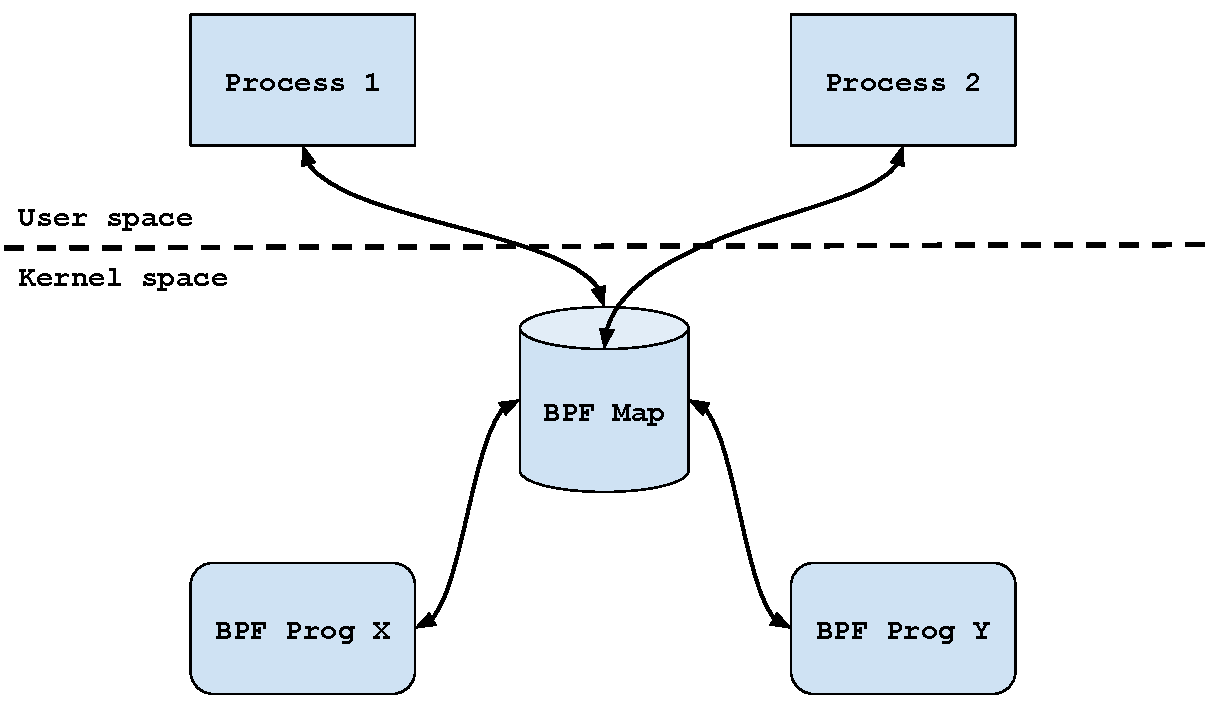
\includegraphics[width=.75\linewidth]{pics/bpf_map}
	\caption{BPF Map}
	\label{fig:bpf-map}
\end{figure}

There are also many map types available as seen in Table~\ref{tab:generic_ebpf_maps} and Table~\ref{tab:non_generic_ebpf_maps}. While each generic map type is functionally different, all the map types use a common set of \ac{BPF} helper functions for lookups, updates, and deletions. When these data structures aren't sufficient, non-generic map types may be used to fill the gaps.

\begin{table}[h]
    \centering
    \begin{tabular}{p{6cm} p{8cm}}
        \toprule
        Generic Map Type & Description \\
        \midrule
        \texttt{BPF\_MAP\_TYPE\_HASH} & Standard hash table. \\
        \texttt{BPF\_MAP\_TYPE\_PERCPU\_HASH} & Per-CPU hash table. \\
        \texttt{BPF\_MAP\_TYPE\_LRU\_HASH}  & Hash table with a Least Recently Used (LRU) eviction policy. \\
        \texttt{BPF\_MAP\_TYPE\_LRU\_PERCPU\_HASH} & Per-CPU Hash table with a per CPU Least Recently Used (LRU) eviction policy. \\
        \texttt{BPF\_MAP\_TYPE\_ARRAY} & Standard array, indexed by integer keys. \\
        \texttt{BPF\_MAP\_TYPE\_PERCPU\_ARRAY} & Per-CPU array. \\
        \texttt{BPF\_MAP\_TYPE\_LPM\_TRIE} & Longest Prefix Match Trie, useful for routing and IP address lookups. \\
        \bottomrule
    \end{tabular}
    \caption{Generic eBPF Map Types}
    \label{tab:generic_ebpf_maps}
\end{table}

\begin{table}[h]
    \centering
    \begin{tabular}{p{6cm} p{8cm}}
        \toprule
        Non-Generic Map Type & Description \\
        \midrule
        \texttt{BPF\_MAP\_TYPE\_XSKMAP} & An array used by XDP programs to redirect network packets to AF\_XDP sockets. \\
        \texttt{BPF\_MAP\_TYPE\_PROG\_ARRAY} & An array that holds pointers to other eBPF programs. Used for complex control flow or "tail calls". \\
        \texttt{BPF\_MAP\_TYPE\_PERF\_EVENT\_ARRAY} & Used for sending data from eBPF programs to user space via the \texttt{perf} subsystem. \\
        \texttt{BPF\_MAP\_TYPE\_CGROUP\_ARRAY} & Used to manage BPF programs attached to cgroups. \\
        \texttt{BPF\_MAP\_TYPE\_STACK\_TRACE} & Captures kernel or user space stack traces for profiling and debugging. \\
        \texttt{BPF\_MAP\_TYPE\_ARRAY\_OF\_MAPS} \newline \texttt{BPF\_MAP\_TYPE\_HASH\_OF\_MAPS} & Maps that hold pointers to other maps, allowing for atomic replacement of entire maps at runtime. \\
        \bottomrule
    \end{tabular}
    \caption{Non-Generic (Specialized) eBPF Map Types}
    \label{tab:non_generic_ebpf_maps}
\end{table}

\subsection{Limitations}
While powerful, \ac{eBPF} isn't a silver bullet. Its capabilities remain significantly more constrained than those of a typical user space application. For example, it doesn't support function calls with six or more arguments, the strict verifier might reject a program if it can't definitively prove termination, and \ac{eBPF} programs have access to only a very limited set of helper functions and a small stack size. Finally, debugging is basic. It is currently not possible to step through an \ac{eBPF} program while it runs in the kernel, which consequently makes print debugging the most effective method. For most use cases, user space applications are still the most viable option.

\section{XDP}
\label{sec:xdp}

\ac{XDP} is a \ac{BPF} hook point early in the network receive path and triggers a run of the \ac{BPF} program for every packet reception. Seen in Figure~\ref{fig:xdp-hook-point}, there exist two \ac{XDP} hook points: \texttt{XDP\_DRV} and \texttt{XDP\_SKB}. The former represents the earliest possible point at which a packet may be processed in software and requires integration within the network driver. The latter represents the earliest point at which a packet may be processed without driver support. 

Figure~\ref{fig:xdp-hook-point}

\begin{figure}
	\centering
	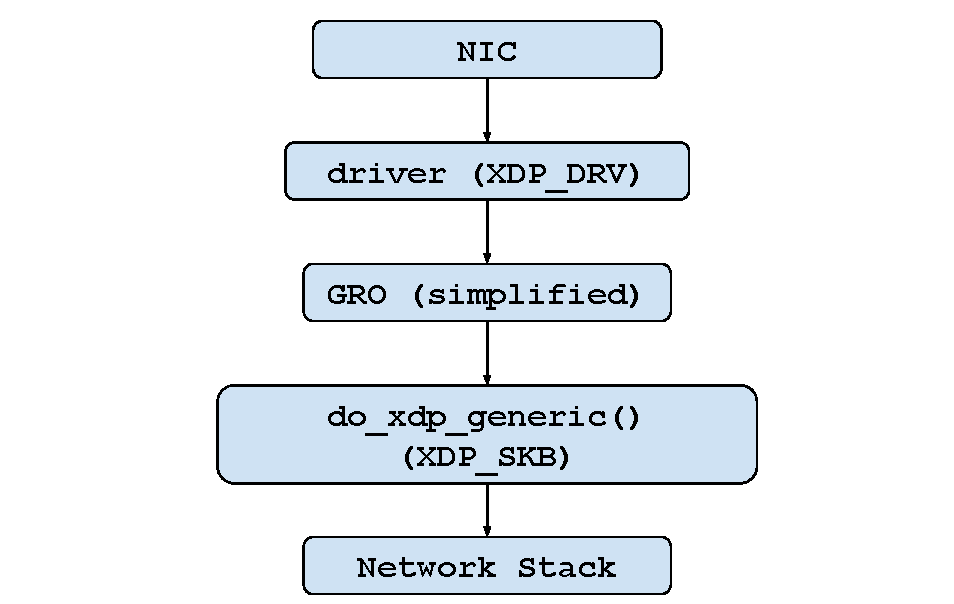
\includegraphics[width=.5\linewidth]{pics/xdp_hook_point}
	\caption{XDP Hook Points}
	\label{fig:xdp-hook-point}
\end{figure}

\section{AF\_XDP}
\label{sec:afxdp}

\section{MsQuic}
\label{sec:msquic}

\section{POS Measurement Framework}
\label{sec:pos-measurement-framework}

% There department-specific \href{https://www.in.tum.de/en/current-students/administrative-matters/thesis-guidelines-and-topics/}{\textcolor{TUMBlue}{guidelines}} that describe the formatting rules and general guidelines for handing in your theses at the \school.

% The Chair for Network Architectures and Services offers additional \href{https://net.in.tum.de/theses/guidelines.pdf}{\textcolor{TUMBlue}{guidelines}} for theses.
